% simon.dobnik@gu.se

\documentclass[a0,36pt,plainsections]{sciposter}
\usepackage{gu-poster}
\usepackage{tikz}
% \usepackage{graphicx}
% \usepackage{subfigure}
% \usepackage{booktabs}
% \usepackage{amsmath}
% \usepackage{amssymb}

% Set up colors
\definecolor{highlightblue}{RGB}{41,128,185}
\definecolor{lightgray}{RGB}{240,240,240}

% Custom commands
\newcommand{\sectiontitle}[1]{\textcolor{highlightblue}{\textbf{\Large #1}}}
\newcommand{\subsectiontitle}[1]{\textcolor{black}{\textbf{\large #1}}}

\title{Learning to Refer: How Scene Complexity Affects \\ \vspace{-2.25cm} Emergent Communication in Neural Agents}

\author{Dominik Künkele$^{1}$ and Simon Dobnik$^{1,2}$}

\institute{
  $^1$Department of Philosophy, Linguistics and Theory of Science \\
  $^2$Centre for Linguistic Theory and Studies in Probability (CLASP) \\
  University of Gothenburg, Sweden
}

\email{contact@dominik-kuenkele.de simon.dobnik@gu.se}

% Conference name in the footer
\conference{IWCS 2025}

% Adjust the font size if necessary

\renewcommand{\titlesize}{\huge}
% \renewcommand{\authorsize}{\Large}
% \renewcommand{\instsize}{\large}

\begin{document}

\maketitle

% Places the logo to the edge of the page

\begin{tikzpicture}[remember picture,overlay]
  \node [anchor=north east] at ([xshift=-6cm,yshift=-2cm]current page.north east) {
\includegraphics[height=8cm]{pics/GU-logo.pdf}};
  % \node [anchor=north east, inner sep=2.5cm] at ([xshift=-4cm,yshift=0cm]current page.north east)     {
\includegraphics[height=8cm]{pics/GU-logo.pdf}}; 
\end{tikzpicture}


\begin{multicols}{3}

  % AIMS
  \section*{\sectiontitle{Aims}}
  \begin{itemize}
    \item Bridge continuous sensory input with discrete linguistic symbols
    \item Study symbol grounding in neural agents through interactive communication
    \item Investigate how scene complexity affects emergent language learning
    \item Examine referring expression generation in controlled visual environments
    \item Compare emergent vs. natural language communication protocols
  \end{itemize}

  % ARCHITECTURE
  \section*{\sectiontitle{Architecture}}
  
  \begin{figure}[h]
    \centering
    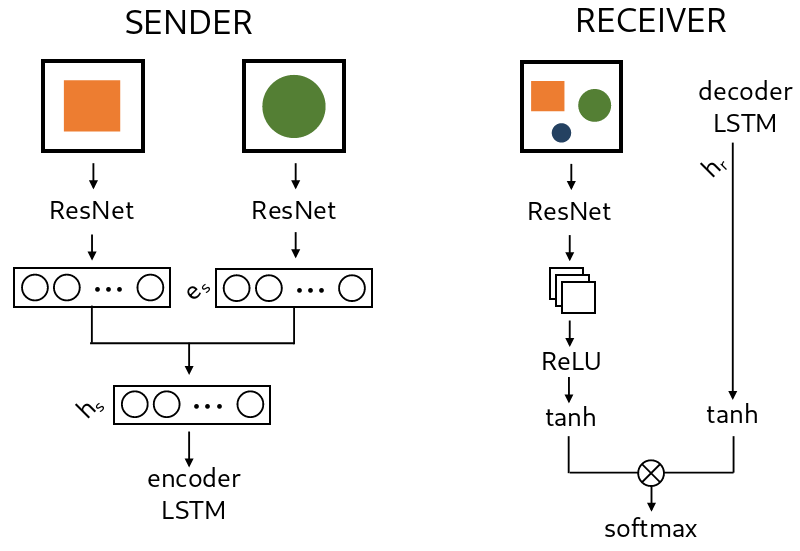
\includegraphics[width=0.95\linewidth]{figures/arch_attention_predictor_game.png}
  \end{figure}
  
  % \textbf{Language Game Setup:}
  % \begin{itemize}
  %   \item \textbf{Sender}: Processes target object features via ResNet-101, generates discrete message using LSTM
  %   \item \textbf{Receiver}: Encodes full scene, interprets message, predicts target location (14×14 attention map)
  %   \item \textbf{Learning}: Gumbel-Softmax relaxation enables end-to-end training through discrete communication
  %   \item \textbf{Evaluation}: Binary cross-entropy loss on 3×3 target regions
  % \end{itemize}

  % CONCLUSIONS
  \section*{\sectiontitle{Conclusions}}
  \begin{itemize}
    \item Medium vocabularies (10-16 symbols) and message lengths (2-4) perform best
    \item Scene complexity dramatically impacts communication success
    \item Shape attributes easiest to learn, size attributes most challenging
    \item Emergent protocols achieve substantial gains over baselines
    \item Natural language bias improves performance significantly
    \item Future: Analyze linguistic properties of emergent languages
  \end{itemize}

\end{multicols}

\vfill

% DATASET RESULTS SECTION
\begin{multicols}{3}
  
  % DALE-2 COLUMN
  \section*{\sectiontitle{Dale-2 Dataset}}
  
  \begin{center}
    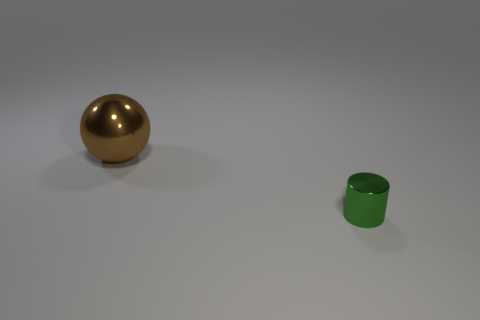
\includegraphics[width=0.9\linewidth]{figures/CLEVR_dale-2.png}\\
    \textit{Target + 1 distractor}
  \end{center}
  
  \begin{center}
    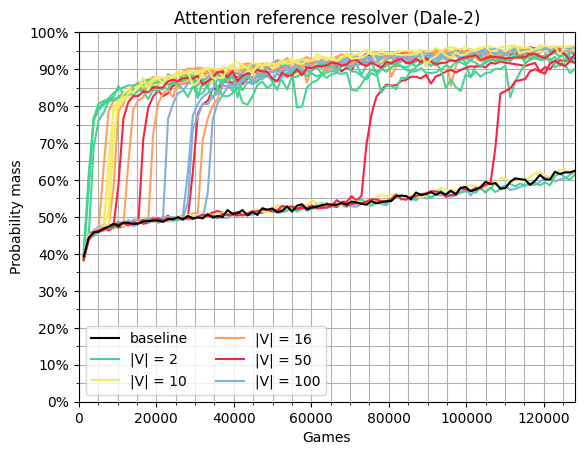
\includegraphics[width=0.9\linewidth]{figures/learning-curve_attention-predictor_dale-2_vocab-size.png}\\
    \textit{Learning curves by vocabulary size}
  \end{center}
  
  \textbf{RE Generation Results:}
  \begin{itemize}
    \item \textbf{Accuracy}: 99\%
    \item \textbf{F1-Score}: 98.57\%
    \item \textbf{Shape}: 99.75\% precision
    \item \textbf{Color}: 98.09\% precision  
    \item \textbf{Size}: 98.73\% precision
  \end{itemize}

  % DALE-5 COLUMN  
  \section*{\sectiontitle{Dale-5 Dataset}}
  
  \begin{center}
    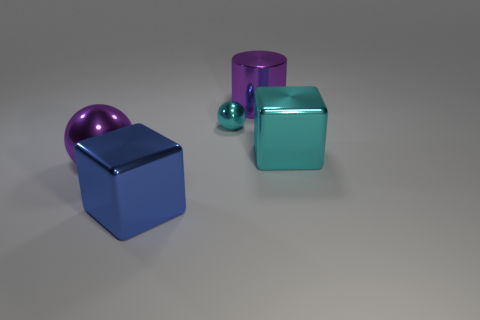
\includegraphics[width=0.9\linewidth]{figures/CLEVR_dale-5.png}\\
    \textit{Target + 4 distractors}
  \end{center}
  
  \begin{center}
    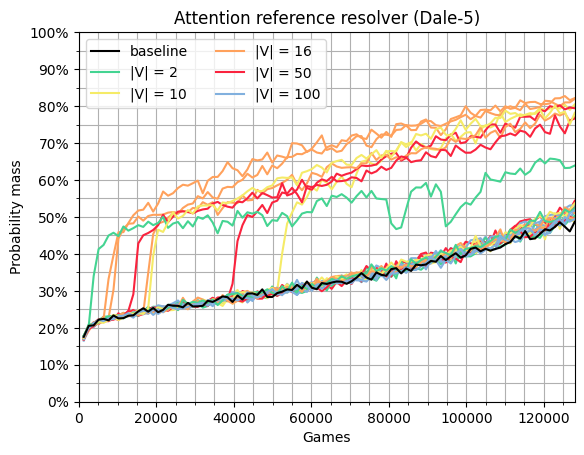
\includegraphics[width=0.9\linewidth]{figures/learning-curve_attention-predictor_dale-5_vocab-size.png}\\
    \textit{Learning curves by vocabulary size}
  \end{center}
  
  \textbf{RE Generation Results:}
  \begin{itemize}
    \item \textbf{Accuracy}: 69\%
    \item \textbf{F1-Score}: 89.53\%
    \item \textbf{Shape}: 98.30\% precision
    \item \textbf{Color}: 92.44\% precision
    \item \textbf{Size}: 69.43\% precision
  \end{itemize}

  % CLEVR COLOR COLUMN
  \section*{\sectiontitle{CLEVR Color Dataset}}
  
  \begin{center}
    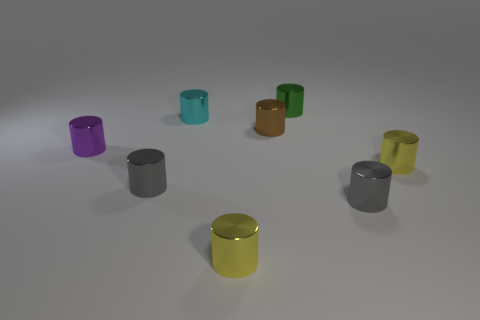
\includegraphics[width=0.9\linewidth]{figures/CLEVR_color.png}\\
    \textit{Target identified by color only}
  \end{center}
  
  \begin{center}
    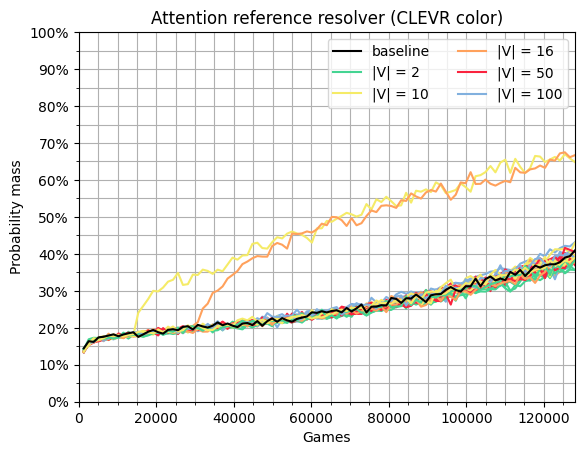
\includegraphics[width=0.9\linewidth]{figures/learning-curve_attention-predictor_colour_vocab-size.png}\\
    \textit{Learning curves by vocabulary size}
  \end{center}
  
  \textbf{RE Generation Results:}
  \begin{itemize}
    \item \textbf{Accuracy}: 93\%
    \item \textbf{F1-Score}: 95.17\%
    \item \textbf{Shape}: 100\% precision
    \item \textbf{Color}: 92.76\% precision
    \item \textbf{Size}: N/A (not used)
  \end{itemize}

\end{multicols}

\vfill



\end{document}

%% \section*{Acknowledgements}





%% Bibliography

\small

\bibliographystyle{acl_natbib}
\bibliography{references.bib}





\end{multicols}


\end{document}



%%% Local Variables:
%%% mode: latex
%%% mode: flyspell
%%% TeX-master: t
%%% TeX-PDF-mode: t
%%% coding: utf-8
%%% ispell-local-dictionary: "british"
%%% End:
